%%%%%%%%%%%%%%%%%%%%%%%%%%%%%%%%%%%%%%%%%
% Journal Article
% LaTeX Template
% Version 1.4 (15/5/16)
%
% This template has been downloaded from:
% http://www.LaTeXTemplates.com
%
% Original author:
% Frits Wenneker (http://www.howtotex.com) with extensive modifications by
% Vel (vel@LaTeXTemplates.com)
%
% License:
% CC BY-NC-SA 3.0 (http://creativecommons.org/licenses/by-nc-sa/3.0/)
%
%%%%%%%%%%%%%%%%%%%%%%%%%%%%%%%%%%%%%%%%%

%----------------------------------------------------------------------------------------
%	PACKAGES AND OTHER DOCUMENT CONFIGURATIONS
%----------------------------------------------------------------------------------------

\documentclass[14pt, a4paper]{article}
\usepackage[english, russian]{babel}
\usepackage{fontspec}
% \setmainfont{Times New Roman}

\setromanfont{Times New Roman}
\setsansfont{Arial}

% \usepackage{cyrtimes}

\usepackage{extsizes}
% \usepackage[T2A]{fontenc}
%
% \usepackage[utf8]{inputenc}

\usepackage{indentfirst}

%\usepackage{times}
\linespread{1.5}
\usepackage[left=30mm,right=15mm,top=15mm,bottom=20mm]{geometry}
\usepackage[framed,numbered,autolinebreaks,useliterate]{mcode}

\usepackage{graphicx, amsmath}
\graphicspath{{images/}}
\usepackage{amsfonts,amssymb}
\usepackage{caption}
\captionsetup[figure]{name=Рисунок, labelsep=endash}
\captionsetup[table]{labelsep=quad}


\usepackage{booktabs} % Horizontal rules in tables

\usepackage{lettrine} % The lettrine is the first enlarged letter at the beginning of the text

\usepackage{enumitem} % Customized lists
\setlist[itemize]{noitemsep} % Make itemize lists more compact

\usepackage{listings}
\usepackage{courier}
\usepackage{tocloft}
\usepackage{array}
\newcolumntype{H}{>{\setbox0=\hbox\bgroup}c<{\egroup}@{}}

\lstloadlanguages{Python}%,Clean,make,Fortran}%Загружаемые языки
\lstset{
	language=Python,                % choose the language of the code
	numbers=left,                   % where to put the line-numbers
	stepnumber=1,                   % the step between two line-numbers.
	numbersep=5pt,                  % how far the line-numbers are from the code
	backgroundcolor=\color{white},  % choose the background color. You must add \usepackage{color}
	showspaces=false,               % show spaces adding particular underscores
	showstringspaces=false,         % underline spaces within strings
	showtabs=false,                 % show tabs within strings adding particular underscores
	tabsize=2,                      % sets default tabsize to 2 spaces
	captionpos=b,                   % sets the caption-position to bottom
	breaklines=false,                % sets automatic line breaking
	breakatwhitespace=false,         % sets if automatic breaks should only happen at whitespace
	frame=none,
	basicstyle=\footnotesize\ttfamily
	%title=\lstname,                 % show the filename of files included with \lstinputlisting;
}

\usepackage{abstract} % Allows abstract customization
\usepackage{braket} % \bra{f}\ket
\usepackage{rotating}
\renewcommand{\abstractnamefont}{\normalfont\bfseries} % Set the "Abstract" text to bold
\renewcommand{\abstracttextfont}{\normalfont\small\itshape} % Set the abstract itself to small italic text
\newcommand{\sectionbreak}{\clearpage}
\newcommand*{\No}{\textnumero}
\renewcommand{\Re}{\mathrm{Re}}
\renewcommand{\Im}{\mathrm{Im}}

\newcommand{\const}{\mathrm{const}}
\newcommand{\arccosh}{\mathrm{arccosh}}

\newcommand{\vF}{\mathbf{F}}
\newcommand{\ve}{\mathbf{e}}
\newcommand{\vk}{\mathbf{k}}
\newcommand{\vq}{\mathbf{q}}
\newcommand{\vp}{\mathbf{p}}
\newcommand{\va}{\mathbf{a}}
\newcommand{\vP}{\mathbf{P}}
\newcommand{\vK}{\mathbf{K}}
\newcommand{\vQ}{\mathbf{Q}}
\newcommand{\vA}{\mathbf{A}}
\newcommand{\vr}{\mathbf{r}}
\newcommand{\vR}{\mathbf{R}}

\newcommand{\vRR}{\boldsymbol{\mathcal{R}}}
\newcommand{\veps}{\boldsymbol{\varepsilon}}

\newcommand{\cA}{\mathcal{A}}
\newcommand{\cR}{\mathcal{R}}
\newcommand{\cM}{\mathcal{M}}
\newcommand{\cE}{\mathcal{E}}
\newcommand{\cJ}{\mathcal{J}}
\newcommand{\cT}{\mathcal{T}}
\newcommand{\cD}{\mathcal{D}}
\usepackage{titlesec} % Allows customization of titles
% \renewcommand\thesection{\Roman{section}} % Roman numerals for the sections
% \renewcommand\thesubsection{\roman{subsection}} % roman numerals for subsections
\titleformat{\section}[block]{\normalsize\bfseries}{\thesection}{1ex}{}
\titleformat{\subsection}[block]{\normalsize\bfseries}{\thesubsection}{1ex}{}

\renewcommand{\cftsecleader}{\cftdotfill{\cftdotsep}}
\cftsetindents{section}{0em}{2em}
\cftsetindents{subsection}{0em}{2em}

\renewcommand\cfttoctitlefont{\hfill\normalsize\bfseries}
\renewcommand\cftaftertoctitle{\hfill\mbox{}}
\renewcommand\labelitemi{---}

\usepackage{hyperref} % For hyperlinks in the PDF

\addto\captionsrussian{\def\refname{Список использованных источников}}
\usepackage{setspace}
\onehalfspacing

\makeatletter
\renewcommand*{\@biblabel}[1]{#1}
\makeatother


\usepackage{titlesec}
\titleformat{\section}[block]{\normalsize\bfseries\centering}{\thesection}{1ex}{}
\titleformat{\subsection}[block]{\normalsize\bfseries}{\thesubsection}{1ex}{}
\titleformat{\subsubsection}[block]{\normalsize\bfseries}{\thesubsubsection}{1ex}{}
\usepackage[tocflat]{tocstyle}
%----------------------------------------------------------------------------------------
%	TITLE SECTION
%----------------------------------------------------------------------------------------


%----------------------------------------------------------------------------------------

\begin{document}
\tableofcontents
\section*{\centering Введение}
\addcontentsline{toc}{section}{Введение}
В данной работе рассматривается синтез ядер в астрофизических процессах. Процессы, приводящие к появлению легких элементов (с массовым числом меньше массового числа $Fe$) относительно известны и изучены. Однако распространенности элементов, тяжелее железа, относительно слабо зависят от массового числа A, что свидетельствует о ином механизме образования этих элементов. Образование такие ядер в результате взаимодействия заряженных частиц сильно подавлено из-за кулоновского барьера. Также большинство тяжелых элементов являются $\beta$-радиоактивными. На данный момент считается, что тяжелые элементы образуются в реакциях захвата нейтронов. Обычно различают быстрый (r) и медленный (s) процессы захвата нейтронов (от английских слов rapid и slow). Эти два механизма различаются отношением скорости захвата нейтронов (реакция (n, $\gamma$)) к скорости бета-распада. Предполагается, что примерно половина наблюдаемого количества элементов с A > 60 образуется в результате s-процесса. В настоящее время общепризнанно, что многие ядра тяжелее железа, включая все ядра тяжелее $^{209}Bi$, образуются в   r-процессе путем быстрого последовательного захвата большого количества нейтронов. Как было сказано выше, для r-процесса характерна высокая скорость захвата нейтронов. Это возможно только при определенных условиях, которые являются экстремальными и встречаются крайне редко. Считается, что такие условия наблюдаются при коллапсировании ядра сверхновых звезд, слиянии нейтронных звезд и при нейтронной звезды черной дырой.

Однако, образование некоторых изотопов не может быть объяснено в рамках указанных выше процессов, эти элементы принято называть обойденными или p-изо\-то\-па\-ми. Их название обусловлено тем, что они являются изотопами с относительным избытком протонов, и, если рассмотреть картину s-процесса и r-процесса, то можно увидеть, что эти стабильные элементы не могут быть получены путем $\beta$-распада, так как в данных условиях, он не является разрешенным.

Несмотря на то, что распространенности обойденных ядер, как правило, на два-три порядка меньше, чем у ядер, полученных в s- и r-процессах, удовлетворительные количественные результаты для распространенностей p-ядер, образованных различными способами в условиях квазиравновесных этапов эволюции звезды, получить не удалось. Поэтому в последнее время стали активно разрабатывать модели образования p-изотопов в условиях r-процесса.

В данной работе моделируются реакции образования химических элементов в процессе поглощения нейтронной звезды черной дырой \cite{bhns1} с учетом столкновительного β-распада как процесса, приводящего к появлению обойденных ядер. Вычисление сечений реакций производится с использованием данных открытой библиотеки REACLIB, в основе которой лежит аппроксимация температурной зависимости сечения специальной функцией, включающей 7 уникальных для каждой реакции параметров \cite{jina}.

Столкновительный бета-распад был впервые предложен в работе \cite{batkin}, объяснение образования обойденных элементов на
основе СБР - в работе \cite{tak}.

В настоящей работе вычислены сечения СБР, индуцированно столкновениями с протонами для ряда изотопов, а также найдены параметры температурной аппроксимации в формате библиотеки REACLIB. Полученные результаты включены в набор реакций, возникающих при поглощении нейтронной звезды черной дырой, и в дальнейшем выполнено моделирование синтеза химических элементов с помощью открытой библиотеки SkyNet \cite{skynet}, написанной Jonas Lippuner, с дополнением ее своим набором реакций.


\section{Проблема происхождения обойденных элементов}

Процессы, приводящие к образованию элементов можно разделить на несколько видов. Большой взрыв привел к появлению водорода ($\sim75\%$ общей массы) и гелия ($\sim25\%$) в промежутке от первых десяти секунд до минуты после большого взрыва, а также некоторое количество дейтерия, $^3H$e и $^7Li$ \cite{Tytler}.
 
 Далее, звезды проходят через несколько стадий горения, которые в конечном счете могут произвести более тяжелые элементы, таке как $^{20}Ne$, $^{24}Mg$, $^{28}Si$ и т. д., вплоть до массового числа А = 56 (когда энергия связи на нуклон (протоны и нейтроны) достигает максимума) \cite{cauldrons, energy, interiors}. Поэтому более тяжелые нуклиды связаны слабее, что означает, нужно добавить энергию, для обеспечения слияние за пределами A = 56 \cite{cauldrons, qse, massive}. Из-за кулоновского барьера распространенность элементов до пика железа намного выше распространенности более тяжелых нуклидов \cite{iron-abu}.
 
 Процессы приводящие к появлению элементов за железным пиком  - захват нейтронов \cite{cauldrons} и $\beta$-распад ядер-продуктов этого распада. В зависимости от того, является ли время $\tau_\beta$ для $\beta$-распада короче или длиннее чем время $\tau_n$ для захвата нейтронов, выделяют r-процесс и s-процесс.
 
 Протекание s-процесса возможно на квазиравновесной стадии эволюции звезды.
 
 R-процесс приводит к появлению элементов с большим массовым числом, однако требует экстремальных условий и места его протекания до сих пор исследуются. Поскольку сечение захвата нейтронов должно быть велико, требуется очень богатая нейтронами среда \cite{places}. Недавние исследования показывают, что коллапс ядра сверхновых, слияние нейтронных, слияние черной дыры - нейтронной звезд являются единственными жизнеспособными кандидатами на места протекания r-процесса \cite{sites, neutrino, nsns, bhns1}. 
 
 Совсем недавно, был обнаружен коллапсар, который также является местом протекания r-процесса \cite{collapsars}.
 
Однако ни r-процесс, ни s-процесс не объясняют происхождение некоторых ядер, так как после нейтронного захвата обычно идет цепочка последовательных $\beta$-распадов, заканчивающихся стабильным изотопом (A, Z). Его стабильность обусловлена тем, что для последующего $\beta$-перехода $(A, Z) \rightarrow (A, Z + 1)$ возникает энергетический порог высотой до 3 МэВ, а иногда и выше. Последующих захват нейтронов также не может дать ядро (A, Z + 2) с увеличенным числом протонов. Такие ядра называют обойденными или p-ядрами. Обойдённые ядра - устойчивые атомные ядра, лежащие в стороне от всех возможных путей образования тяжёлых ядер из более лёгких в процессе последовательного захвата последними нейтронов \cite{reactions}. Распространённость обойденных ядер, как правило, примерно на два порядка величины ниже, чем у близких к ним ядер, лежащих на пути нейтронного захвата. К таковым относятся: $^{74}Se$, $^{78}Kr$, $^{80}Kr$, $^{84}Sr$, $^{92}Mo$, $^{94}Мо$, $^{96}Ru$, $^{98}Ru$, $^{102}Pd$, $^{106}Cd$, $^{108}Cd$, $^{113}In$, $^{112}Sn$, $^{114}Sn$, $^{115}Sn$, $^{120}Te$, $^{124}Xe$, $^{126}Xe$, $^{130}Ba$, $^{132}Ba$, $^{136}Ce$, $^{138}Ce$, $^{144}Sm$, $^{152}Gd$, $^{152}Dy$, $^{158}Dy$, $^{162}Er$, $^{164}Er$, $^{168}Yb$, $^{174}Hf$, $^{180}W$, $^{184}Os$, $^{190}Pt$, $^{196}Hg$ \cite{role}. Их происхождение до сих пор до конца не изучено \cite{p-process}.

\section{SkyNet}

Программный пакет SkyNet представляет собой бесплатную современную сеть ядерных реакций с открытым исходным кодом \cite{skynet}. Первоначально SkyNet разрабатывался с целью моделирования синтеза ядер в моделях r-процесса, включающих тысячи изотопов и более 100000 реакций, однако благодаря модульной архитектуре и гибкости, данное программное обеспечение может быть использовано для более общих задач астрофизики. 

SkyNet имеет возможность моделировать эволюцию системы из произвольного набора изотопов под действием любых ядерных реакций. В качестве библиотеки ядерных реакций в данном программном обеспечении используются данные формата открытой базы реакций JINA REACLIB. Данная база хранит параметры реакций, такие как зависимость от температуры через семи-параметрическое приближение \cite{jina}, тип реакции (резонирующая, нерезонирующая, слабая, спонтанный распад), значение температуры, переданное среде, а также параметр $v$, указывающий, являются ли показатели $a_0, .., a_6$ обратными. В подавляющем большинстве реакций показатели представляют из себя параметризацию сечения в зависимости от температуры:

\begin{equation}
\label{eq:system}
\begin{split}
\left.
\begin{array}{ccc}
N_{A}\langle \sigma v \rangle \\
\lambda_\gamma
\end{array}
\right\}
= \exp (a_0 + a_1 T_9^{-1} + a_2 T_9^{-1/3} + \\
a_3 T_9^{1/3} + a_4 T_9 + a_5 T_9^{5/3} + a_6 \ln T_9)
\end{split}
\end{equation}

При моделировании ядерных процессов SkyNet может моделировать систему в ядерном статистическом равновесии (NSE) и изменять способ моделирования системы между NSE и полным набором реакций автоматически. Включенные в SkyNet поправки для экранирований электронов и уравнение состояния, учитывающее общую картину эволюции.

В результате работы программного пакета, можно получить обширную информацию о составе исследуемой модели, а именно: температуру, центральную плотность, энтропию, относительные распространенности изотопов и элементарных частиц, их массовые доли и т д. 

\section{Столкновительный β-распад}
Столкновительный $\beta$-распад является одним из процессов, приводящих к появлению обойденных ядер. Впервые он был предложен в работе \cite{batkin}. 

Столкновительный $\beta-$распад стабильных ядер, инициируемый их кулоновскими столкновениями с другими ядерными частицами звездной среды, может быть основой модели процесса синтеза обойденных ядер.
Проблема их синтеза на основе физического механизма захвата нейтронов ($s-$ или $r-$процесса) состоит в прерывании цепочки последовательных $\beta-$распадов на $\beta$-стабильном ядре $(A,Z)$.

Процесс СБР стабильных ядер, о котором говорилось выше, для нуклидов главной последовательности предоставляет еще одну возможность преодолеть энергетический порог и осуществить переход 
$$(A,Z) \xrightarrow[]{\beta^-} (A,Z + 1),$$
открывая путь к последующему естественному $\beta$-переходу
$$(A,Z+1) \xrightarrow[]{\beta^-} (A,Z + 2).$$

Расчеты показывают, что модель синтеза обойденных элементов в звездном веществе на этапе квазиравновесной стадии, основанная на явлении СБР стабильных ядер главной последовательности, качественно способна воспроизвести нерегулярный ход кривой относительной распространенности обойденных ядер. Этот факт можно расценивать как косвенное свидетельство в пользу реальности явления столкновительного $\beta$-распада стабильных ядер \cite{tak}.

В случае столкновительного $\beta$-распада возможно несколько видов процессов, а именно: протон-ядерные, ядро-ядерные и процесс, стимулированный нейтронами. Мы рассмотрим $\beta$-распад, стимулированных столкновением с протонами. Рассчитанные сечения для протон-ядерных и ядро-ядерных оказались невелики (менее $10^{-50}cm^2$), и процесс пока не доступен для прямого наблюдения, но при помощи программного обеспечения, позволяющего моделировать данные процессы мы можем оценить влияние их на конечные распространенности элементов в звездном веществе \cite{tak_article}.

Сечение для столкновительного $\beta$-распада при столкновении частицы с протоном или другой частицей имеет вид:
\begin{equation} \label{sech}
\langle\sigma \cdot v\rangle = \left(\frac{8}{\pi\mu T^3}\right)^{1/2} \int_{\Delta + \Delta_f + 1} \sigma^{(col)}_\beta(\beta_f) \exp(-\varepsilon/T)d\varepsilon,
\end{equation}
где  
\begin{multline} \label{sig}
\sigma^{(col)}_\beta(\beta_f)=
{4\sqrt{2}\over \pi} {{g^2_v\alpha_e^4Z (Z+1) {Z'}^4 \mu^{9/2}}
	\over{\varepsilon_i^{3/2} (1-exp(-2\pi\lambda_i))}}
\xi_\beta(\beta_f)
\times\\
\times\int\limits_0^{\varepsilon_i{-}\Delta{-}\Delta_f}\!\!\!\!\!
{{\Phi(E_f) d\varepsilon_f}\over{(exp(2\pi\lambda_f)-1)
		k_f ( k_i- k_f)^4(k_i+k_f)^2}}\times\\
\times\int\limits_{x_0}^0 {{|{\rm F}(-i \lambda_i, -i\lambda_f,1; x)|^2}\over{(1-x)^2}} dx,
\end{multline}
$$
x_0=-4 k_i k_f/(k_i- k_f)^2,
$$
$$
\Phi (E)={1\over 60}(E^2-1)^{1/2}(2E^4-9E^2-8)+{1\over 4}E\ln{(E+(E^2-1)^{1/2})},
$$
$$
E_f=\varepsilon_i-\varepsilon_f-\Delta-\Delta_f,
$$
$$
\lambda_i = {Z Z' e^2 \mu\over {\hbar}^2 k_i},
\lambda_f = {(Z+1) Z' e^2 \mu\over \hbar^2 k_f}.
$$
Индекс $i$ соответствует начальному состоянию столкновительной системы, $f$ - конечному.$k_s$ - относительный импульс в $s$-м состоянии, $\mu$ - приведенная масса системы. $\Delta$ -пороговая энергия, определяемая разностью энергий связи дочернего и материнского ядер, $\Delta_f$ - ???, $\alpha_e$ - постоянная тонкой структуры, $g_v$ - постоянная слабого взаимодействия, $\varepsilon_s$ - ???,
\section{Постановка задачи r-процесса}

Целью данной работы является оценка вклада столкновительного $\beta$-распада на происхождение обойденных элементов. Для этого смоделируем при помощи SkyNet слияние черной дыры и нейтронной звезды (BHNS) с использование заранее известных параметров системы \cite{bhns}.

Начальный состав представляет из себя $T = 6.1 \text{ГК}$, $\rho = 7.4 \times 10^9 \text{г} \text{см}^{-3}$, и $Y_e = 0.07$ ($T$ -- температура, $\rho$ -- центральная плотность, $Y_e$ -- относительная концентрация электронов). В данной работе мы выбрали именно эту систему для моделирования образования обойденных элементов в процессе столкновительного $\beta$-распада, индуцированного столкновениями с протонами. Эволюция данного процесса протекает на отрезке времени от $10^{-3}\text{с}$ до $5\times10^8\text{с}$.

Для непосредственной оценки влияний СБР рассчитаем сечения реакций, приводящий к появлению обойденных элементов, параметризуем их для приведения к формату JINA REACLIB и добавим в сеть.

В конечном итоге сравним распространенности обойденных элементов с учетом СБР и без его учета.

\section{Аппроксимация}

Были рассчитаны сечения столкновительного $\beta$-распада некоторых элементов с протоном. Для мы этого воспользовались параметрами из таблицы \ref{Tels}. 

\begin{table}
	\centering
	\caption{Характеристики праматеринских ядер.}
	\tabcolsep=5pt
	\begin{tabular}{|c|c|c|HHc|c|}
		\hline
		Праматеринское& Материнское & Обойденное &$\; J_i\; $&$J_f$&$\Delta + \Delta_f,$&${\rm lg} f_0t$\\
		ядро  &   ядро & ядро &&&$\text{МэВ}$&\\
		\hline
		$^{74}Ge$ & $^{74}As$ &$^{74}Se$ & $0^+$  &  $(1^+)$ & 2,766 &      \\
		$^{74}Ge$ & $^{74}As$ &$^{74}Se$& $0^+$  &  $(1^+)$ & 2,982 &      \\
		$^{78}Se$ & $^{78}Br$ &$^{78}Kr$& $0^+$  &  $1^+$  & 3,5737 &   4,8   \\
		$^{80}Se$ & $^{80}Br$ &$^{80}Kr$& $0^+$  &  $1^+$  & 1,8703 &   4,6  \\
		$^{84}Kr$ & $^{84}Rb$ &$^{84}Sr$& $0^+$  &  $2^-$  & 2,68   &   9,6  \\
		$^{106}Pd$ & $^{106}Ag$ &$^{106}Cd$& $0^+$  &  $1^+$  & 2,983 &   4,9   \\
		$^{106}Pd$ & $^{106}Ag$ &$^{106}Cd$& $2^+$  &  $1^+$  & 2,471 &   5,3   \\
		$^{108}Pd$ & $^{108}Ag$ &$^{108}Cd$& $0^+$  &  $1^+$  & 1,921 &   4,8   \\
		$^{108}Pd$ & $^{108}Ag$ &$^{108}Cd$& $2^+$  &  $1^+$  & 1,487 &   5,5   \\
		$^{112}Cd$ & $^{112}In$ &$^{112}Sn$& $0^+$  &  $1^+$  & 2,578 &   4,7   \\
		$^{112}Cd$ & $^{112}In$ &$^{112}Sn$& $2^+$  &  $1^+$  & 1,961 &   5,3   \\
		$^{114}Cd$ & $^{114}In$ &$^{114}Sn$& $0^+$  &  $1^+$  & 1,9846 &   4,8   \\
		$^{114}Cd$ & $^{114}In$&$^{114}Sn$ & $2^+$  &  $1^+$  & 1,4266 &   5,3   \\
		$^{120}Sn$ & $^{120}Sb$ &$^{120}Te$& $0^+$  &  $1^+$  & 2,681 &   4,5   \\
		$^{124}Te$ & $^{124}I$  &$^{124}Xe$& $0^+$  &  $2^-$  & 3,157 &   9,3   \\
		$^{124}Te$ & $^{124}I$  &$^{124}Xe$& $2^+$  &  $2^-$  & 2,555 &   7,5   \\
		$^{126}Te$ & $^{126}I$  &$^{126}Xe$& $0^+$  &  $2^-$  & 2,156 &   9,2   \\
		$^{126}Te$ & $^{126}I$ &$^{126}Xe$ & $2^+$  &  $2^-$  & 1,49 &   7,4   \\
		$^{130}Xe$ & $^{130}Cs$ &$^{130}Ba$& $0^+$  &  $1^+$  & 3,019 &   5,1   \\
		$^{130}Xe$ & $^{130}Cs$ &$^{130}Ba$& $2^+$  &  $1^+$  & 2,483 &   6,4   \\
		$^{132}Xe$ & $^{132}Cs$ &$^{132}Ba$& $2^+$  &  $2^{(-)}$  & 1,443 &   6,0   \\
		$^{136}Ba$ & $^{136}La$ &$^{136}Hf$& $0^+$  &  $1^+$  & 2,87 &   4,6   \\
		$^{164}Dy$ & $^{164}Ho$ &$^{164}Er$& $0^+$  &  $1^+$  & 1,0292 &   4,6   \\
		$^{164}Dy$ & $^{164}Ho$ &$^{164}Er$& $2^+$  &  $1^+$  & 0,9558 &   4,9   \\
		\hline
	\end{tabular}
	\label{Tels}
\end{table}

Полученные сечения для переходов можно видеть на рисунке \ref{ris:sigma-full}.

\begin{figure}[ht]
	\center{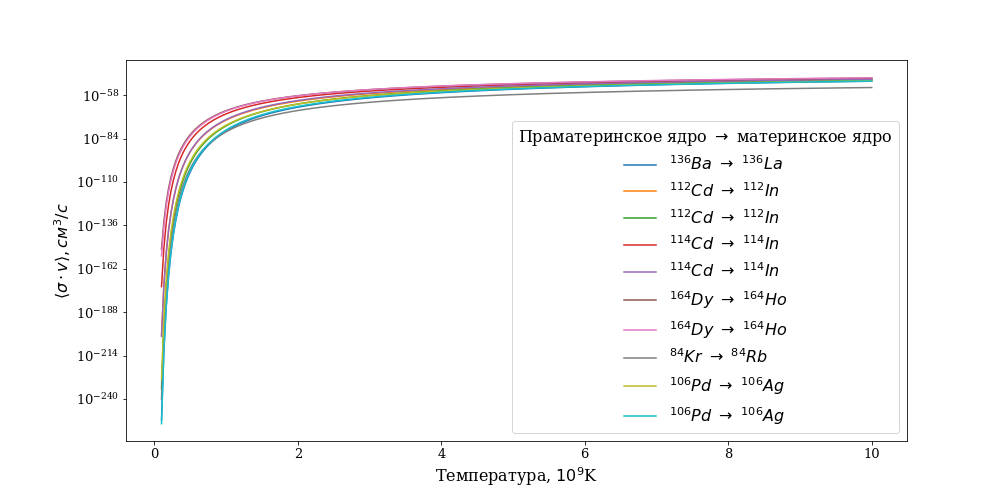
\includegraphics[width=1\linewidth]{article-img/sigma-full}}
	\caption{Сечение столкновительного $\beta$-распада при столкновении ядер ($^{136}Ba, \ ^{112}Cd, \ ^{114}Cd, \ ^{164}Dy, \ ^{84}Kr, \ ^{106}Pd$) с протоном}
	\label{ris:sigma-full}
\end{figure}

Сечение каждой реакции были посчитаны для набора из 24 температур: $T_9$ = 0.1,0.15, 0.2, 0.3, 0.4, 0.5, 0.6, 0.7, 0.8, 0.9, 1.0, 1.5, 2.0, 2.5, 3.0, 3.5, 4.0, 4.5, 5.0, 6.0, 7.0, 8.0, 9.0, 10.0 ($T = T_9 \times 10^{9}\text{К}$). Так как данный набор является избыточным для параметризации вида \ref{eq:system}, был использован метод наименьших квадратов. 

\begin{figure}[ht]
	\center{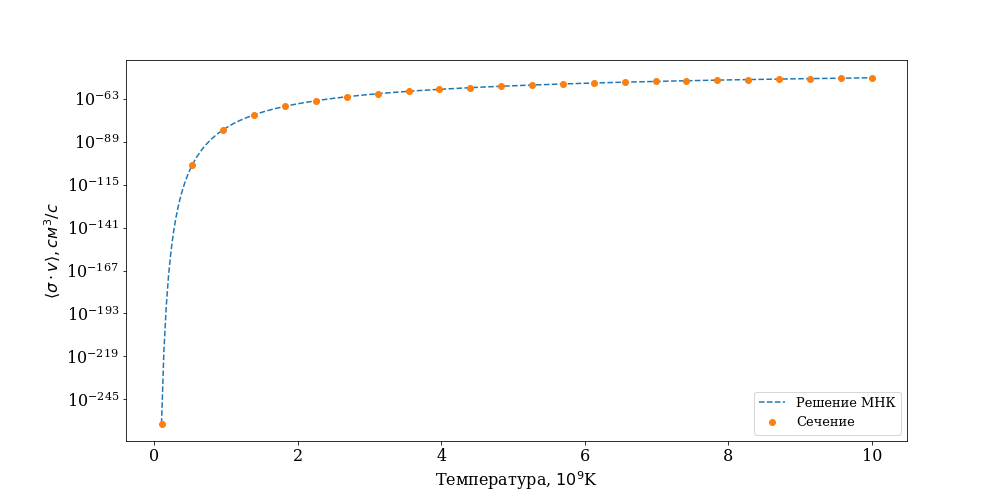
\includegraphics[width=1\linewidth]{article-img/compare-xe130-cs130}}
	\caption{Сравнение решения методом наименьших квадратов с рассчитанным сечением}
	\label{ris:2}
\end{figure}

Далее, был составлен необходимый для REACLIB файл библиотеки реакций. Для перехода $^{130}Xe \to \ ^{130}Cs$ получаем строки вида: 

\begin{lstlisting}[label={lst:label}]
5
pxe130cs130    p                  cleaw     0.00000e+00          
3.631089e+01-2.513083e+01-3.379005e+02 1.434772e+02                      
-2.028014e+00-6.306473e-02-1.208779e+02                                   

\end{lstlisting}


\section{Анализ результатов}

\begin{figure}[ht]
	\center{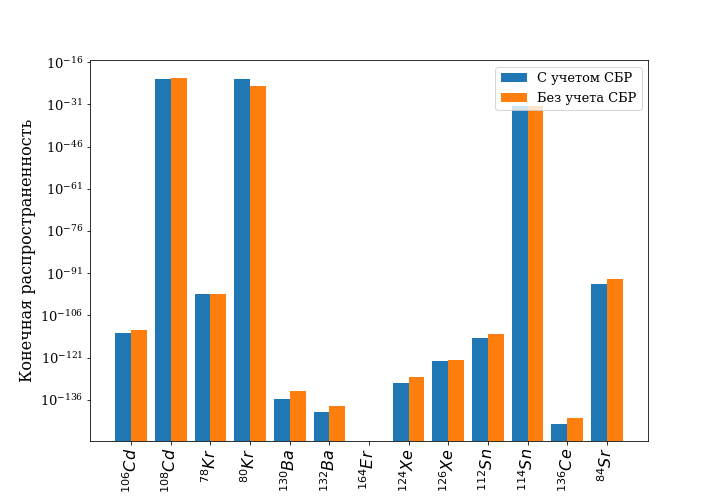
\includegraphics[width=1\linewidth]{article-img/result}}
	\caption{Конечные распространенности обойденных ядер с исходной библиотекой (синий график), и библиотекой, включающей СБР (розовой график)}
	\label{ris:result}
\end{figure}

Самым важным на данном графике является то, что, несмотря на ожидание увидеть меньшие распространенности всех элементов, мы наблюдаем то, что для некоторых ядер это разница несущественна $^{114}Sn$. Более того, наблюдается относительный избыток ядер $^{78}Kr$ и $^{80}Kr$.

\section*{\centering Заключение}
\addcontentsline{toc}{section}{Заключение}
В данной работе было рассмотрено влияние столкновительного бета-распада на синтез тяжелых изотопов в звездном веществе.

Были вычислены сечения столкновительного $\beta$-распада для химических элементов из таблицы \ref{Tels}, а именно, рассматривались столкновения праматеринских ядер с протоном. 

Полученные сечения были параметризированны через 7 параметров $a_0, ..., a_6$, определяющих зависимость от температуры, чтобы иметь возможность дополнить реакциями библиотеку JINA REACLIB. Из полученных наборов параметров, был построен файл, содержащий сеть реакций столкновительного $\beta$-распада, индуцированного столкновением с протоном для последующего использования в пакете SkyNet.


Далее, при помощи пакета SkyNet было проведено моделирование слияние черной дыры-нейтронной звезды, чтобы оценить влияние СБР на общую картину распространенностей элементов. Моделирование проводилось дважды, сначала - с немодифицированной библиотекой JINA REACLIB, затем - с модифицированной, в которую были включены реакции $$\text{праматеринское ядро} \to \text{материнское ядро}.$$

Было выполнено сравнение полученных картин распространенностей элементов.  Сравнение производилось для обойденных элементов, так как именно их происхождения является целью данной работы. Было подтверждено, что СБР может являться источником обойденных ядер и при больших концентрациях протонов (в условиях рассматриваемого процесса) это влияние суще-ственно, более того, мы можем получить даже избыток некоторых элементов.

В данной работе рассматривалось образование материнских ядер только при столкновениях с протонами. 

СБР, индуцированный столкновением с нейтронами, представляет особый интерес, так отсутствие кулоновского барьера существенно увеличивает сечение процесса. Учитывая также, что в рассматриваемых условиях большую часть вещества составляют нейтроны ($\sim 79\%$), окончательный результат может существенно увеличиться, если рассчитать суммарный выход обойденных ядер в модели, основанной на физическом механизме СБР. Поэтому дальнейшее развитие предложенной модели является перспективным.
\newpage
\addcontentsline{toc}{section}{Список используемой литературы}
\bibliographystyle{ugost2003}
\bibliography{sample}

\end{document} 